\section{Understanding the Backward LSTM}\label{sec:backward_lstm}

The inference network needs, at each time step $t$, a summary of the
future observations $\mathbf{x}_{t:T}$. A backward RNN provides all of
them in a single pass.

\subsection*{Definition}

A backward LSTM is an ordinary LSTM run from $t = T$ down to $t = 1$. Its
state at time $t$ is computed from the observation $\mathbf{x}_t$ and the
state at time $t+1$:
\begin{align*}
    \mathbf{f}_t &= \sigma(\mathbf{W}_f [\mathbf{b}_{t+1}, \mathbf{x}_t]
    + \mathbf{c}_f) & &\text{(forget gate)}\\
    \mathbf{i}_t &= \sigma(\mathbf{W}_i [\mathbf{b}_{t+1}, \mathbf{x}_t]
    + \mathbf{c}_i) & &\text{(input gate)}\\
    \tilde{\mathbf{m}}_t &= \tanh(\mathbf{W}_m [\mathbf{b}_{t+1},
    \mathbf{x}_t] + \mathbf{c}_m) & &\text{(candidate memory)}\\
    \mathbf{m}_t &= \mathbf{f}_t \odot \mathbf{m}_{t+1} + \mathbf{i}_t
    \odot \tilde{\mathbf{m}}_t & &\text{(memory cell)}\\
    \mathbf{o}_t &= \sigma(\mathbf{W}_o [\mathbf{b}_{t+1}, \mathbf{x}_t]
    + \mathbf{c}_o) & &\text{(output gate)}\\
    \mathbf{b}_t &= \mathbf{o}_t \odot \tanh(\mathbf{m}_t) & &
    \text{(output)}
\end{align*}
with initial values $\mathbf{b}_{T+1} = \mathbf{0}$ and
$\mathbf{m}_{T+1} = \mathbf{0}$. Here $\sigma$ is the logistic sigmoid,
$[\cdot, \cdot]$ denotes concatenation, and the $\mathbf{W}$'s and
$\mathbf{c}$'s are learned weights and biases.

\begin{inwords}
Unrolling the recursion, $\mathbf{b}_t$ is a function of
$\mathbf{x}_t, \mathbf{x}_{t+1}, \dots, \mathbf{x}_T$ only. So
$\mathbf{b}_t$ summarises exactly the suffix $\mathbf{x}_{t:T}$ that the
posterior factor $q_\phi(\mathbf{z}_t \mid \mathbf{z}_{t-1},
\mathbf{x}_{t:T})$ needs. At $t = T$ it has seen only $\mathbf{x}_T$, and
at $t = 1$ it has seen the whole sequence.
\end{inwords}

\subsection*{Implementation by flipping}

Deep-learning libraries implement LSTMs that run forwards in time. The
backward LSTM is obtained by flipping the sequence, running a forward
LSTM, and flipping the outputs back:
\begin{enumerate}
    \item flip: $(\mathbf{x}_T, \mathbf{x}_{T-1}, \dots, \mathbf{x}_1)$;
    \item run the LSTM: its $k$-th output, $k = 1, \dots, T$, has seen
    $\mathbf{x}_T, \dots, \mathbf{x}_{T-k+1}$;
    \item flip the outputs back: the output now stored at position
    $t = T - k + 1$ has seen $\mathbf{x}_{t:T}$, i.e.\ it is
    $\mathbf{b}_t$.
\end{enumerate}
This is what \code{DKF\_Backward\_RNN} does, with
\code{torch.flip} along the time dimension (dimension 0, since tensors
have shape \code{(seq\_len, batch\_size, dim)}).

\begin{figure}[ht!]
    \centering
    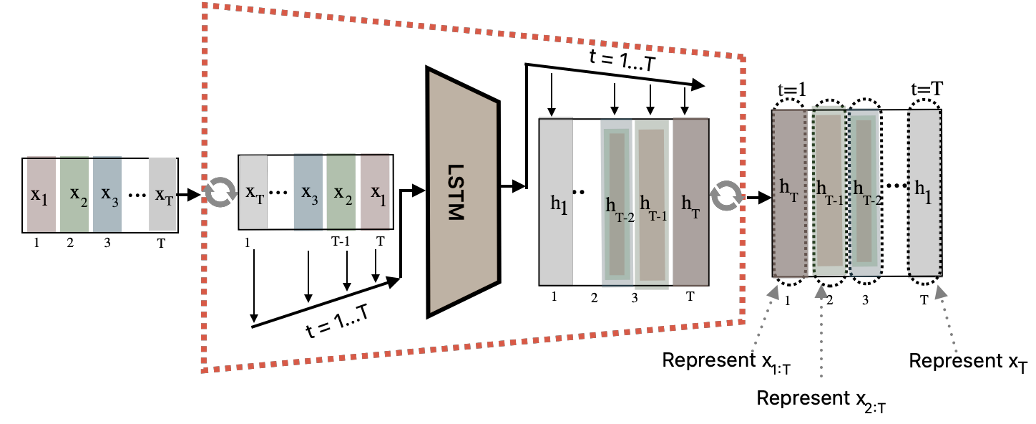
\includegraphics[width=400px]{./Images/backward_lstm.png}
    \caption{Backward LSTM. In this figure the hidden states are indexed
    by their position in the \emph{flipped} sequence: $h_k$ is
    $\mathbf{b}_{T-k+1}$ in the notation of this appendix.}
    \label{fig:backward_lstm}
\end{figure}

